%!TEX TS-program = pdflatex
%!TEX encoding = UTF-8 Unicode
% =============================================================================
%  P1_bernoulli_supp.tex   --  Supplementary Material
%  Compile BEFORE the main paper (see main paper header).
% =============================================================================
\documentclass[bj,authoryear]{imsart}

\usepackage{amsmath,amssymb,mathtools}
\usepackage{bm}
\usepackage{booktabs}
\usepackage{array}
\usepackage{multirow}
\usepackage{enumitem}
\usepackage{graphicx}
\usepackage{float}
\usepackage{nicefrac}
\usepackage{microtype}
\startlocaldefs

\theoremstyle{plain}
\newtheorem{theorem}{Theorem}[section]
\newtheorem{proposition}[theorem]{Proposition}
\newtheorem{lemma}[theorem]{Lemma}
\newtheorem{corollary}[theorem]{Corollary}
\theoremstyle{definition}
\newtheorem{definition}[theorem]{Definition}
\newtheorem{example}[theorem]{Example}
\newtheorem{remark}[theorem]{Remark}
\newtheorem{assumption}[theorem]{Assumption}

\newcommand{\E}{\mathbb{E}}
\newcommand{\Prob}{\mathbb{P}}
\newcommand{\R}{\mathbb{R}}
\newcommand{\N}{\mathbb{N}}
\newcommand{\F}{\mathcal{F}}
\newcommand{\G}{\mathcal{G}}
\newcommand{\A}{\mathcal{A}}
\newcommand{\Z}{\mathcal{Z}}
\newcommand{\Tsig}{\mathcal{T}_\infty}
\newcommand{\norm}[1]{\left\lVert #1 \right\rVert}
\newcommand{\abs}[1]{\left| #1 \right|}
\newcommand{\inner}[2]{\langle #1,\, #2 \rangle}
\newcommand{\given}{\mid}
\newcommand{\iid}{\overset{\mathrm{iid}}{\sim}}
\DeclareMathOperator{\Var}{Var}
\DeclareMathOperator{\Cov}{Cov}
\DeclareMathOperator*{\argmin}{arg\,min}
\newcommand{\od}[1]{\overset{d}{#1}}

\endlocaldefs

% Cross-references to main paper (inlined from P1_main_xrefs.tex)
\makeatletter
\expandafter\def\csname r@cor:ls\endcsname{{2.11}{6}{Approximate local stationary decomposition}{theorem.2.11}{}}
\expandafter\def\csname r@eq:Mbound\endcsname{{1}{4}{MDS Decomposition with Stabilization Rate}{equation.2.1}{}}
\expandafter\def\csname r@eq:Mstab\endcsname{{2}{4}{MDS Decomposition with Stabilization Rate}{equation.2.2}{}}
\expandafter\def\csname r@eq:local-approx-bound\endcsname{{7}{6}{Approximate local stationary decomposition}{equation.2.7}{}}
\expandafter\def\csname r@cor:fclt\endcsname{{2.8}{5}{Functional CLT for MDS innovations}{theorem.2.8}{}}
\expandafter\def\csname r@cor:dim\endcsname{{3.5}{7}{Dimension-stable ARL}{theorem.3.5}{}}
\expandafter\def\csname r@eq:nondeg\endcsname{{5}{4}{MDS Decomposition with Stabilization Rate}{equation.2.5}{}}
\expandafter\def\csname r@lem:equiv\endcsname{{2.1}{3}{Equivalence of forward and tail limits}{theorem.2.1}{}}
\expandafter\def\csname r@prop:predresid\endcsname{{2.9}{5}{Bayes prediction residuals are martingale differences}{theorem.2.9}{}}
\expandafter\def\csname r@sec:empirical\endcsname{{4}{8}{Empirical Studies and Discussion}{section.4}{}}
\expandafter\def\csname r@sec:nonstationary\endcsname{{2.3}{6}{Extension to Non-Stationary Processes}{subsection.2.3}{}}
\expandafter\def\csname r@sec:theory\endcsname{{2}{2}{Methodology}{section.2}{}}
\expandafter\def\csname r@thm:arl\endcsname{{3.2}{7}{In-control ARL lower bound for the Innovation CUSUM}{theorem.3.2}{}}
\expandafter\def\csname r@thm:mds\endcsname{{2.5}{4}{MDS Decomposition with Stabilization Rate}{theorem.2.5}{}}
\makeatother

% =============================================================================
\begin{document}

\begin{frontmatter}
\title{Supplementary Material for:\\[0.3em]
  Martingale Innovations from Contractive Recurrent Networks
  and Dimension-Robust Change-Point Detection}
\runtitle{Supplementary Material}
\author{\inits{Y.-C.\,I.}\fnms{Yuan-chin Ivan}~\snm{Chang}}
\end{frontmatter}

% Reset section/equation counters to A, B, C style for appendix
\setcounter{section}{0}
\renewcommand{\thesection}{\Alph{section}}
\renewcommand{\theequation}{\Alph{section}.\arabic{equation}}
\renewcommand{\thetable}{\Alph{section}.\arabic{table}}
\renewcommand{\thefigure}{\Alph{section}.\arabic{figure}}
\renewcommand{\thetheorem}{\Alph{section}.\arabic{theorem}}

% =============================================================================
\section{Background and Preliminaries}
\label{app:background}

We work throughout on a complete probability space $(\Omega, \A, \Prob)$.
All convergence statements are in the almost-sure or $L^p$ sense unless otherwise noted.

\subsection{Filtrations and the Information Flow}

\begin{definition}[Filtration and natural filtration]
\label{def:filtration}
  A \emph{filtration} is an increasing family of sub-$\sigma$-algebras
  $\F_1 \subseteq \F_2 \subseteq \cdots \subseteq \A$.
  For a sequence $(X_t)_{t\geq 1}$ of random variables, the
  \emph{natural filtration} is $\F_t = \sigma(X_1, \ldots, X_t)$ and its
  completion $\F_\infty^+ = \sigma\bigl(\bigcup_{t\geq 1}\F_t\bigr)$.
\end{definition}

A \emph{decreasing filtration} (or \emph{reverse filtration}) is a family
$\G_1 \supseteq \G_2 \supseteq \cdots$ of sub-$\sigma$-algebras.
The canonical example relevant to this paper is
\begin{equation}
  \G_n = \sigma(X_n, X_{n+1}, \ldots),
  \label{eq:reverse-filtration}
\end{equation}
which formalizes the information contained in the \emph{tail} of the sequence
starting at index $n$.

\begin{definition}[Tail $\sigma$-algebra]
\label{def:tail}
  The \emph{tail $\sigma$-algebra} of a sequence $(X_t)_{t\geq 1}$ is
  \[
    \Tsig = \bigcap_{n=1}^\infty \sigma(X_n, X_{n+1}, \ldots)
           = \bigcap_{n=1}^\infty \G_n.
  \]
  An event $A \in \Tsig$ is \emph{tail-measurable}: its occurrence or
  non-occurrence is not affected by any finite initial segment of the sequence.
\end{definition}

\begin{example}[Tail-measurable functionals]
  For an i.i.d.\ or ergodic sequence $(X_t)$:
  (a) the limit $\lim_{n\to\infty} n^{-1}\sum_{t=1}^n X_t$ (when it exists)
      is $\Tsig$-measurable;
  (b) the event $\{\limsup_{t\to\infty} X_t > c\}$ is tail-measurable;
  (c) the population mean $\mu = \E[X_1]$ is a constant, hence trivially
      $\Tsig$-measurable under any probability measure.
  Finite-dimensional functions of $(X_1,\ldots,X_k)$ for fixed $k$ are
  \emph{not} tail-measurable in general.
\end{example}

\subsection{Martingales and Reverse Martingales}

\begin{definition}[Martingale and martingale difference sequence]
\label{def:martingale}
  A sequence $(M_t, \F_t)_{t\geq 1}$ is a \emph{martingale} if
  $\E[\abs{M_t}] < \infty$ and $\E[M_{t+1}\given\F_t] = M_t$ a.s.\ for all $t$.
  The sequence $(D_t)_{t\geq 1}$ is a \emph{martingale difference sequence} (MDS)
  if $\E[\abs{D_t}] < \infty$ and $\E[D_t\given\F_{t-1}] = 0$ a.s.\ for all $t\geq 2$.
\end{definition}

The posterior mean $\E[\theta\given\F_t]$, for a fixed integrable parameter
$\theta$ and observations $X_1, X_2, \ldots$, is the canonical martingale in
Bayesian sequential analysis.

\begin{definition}[Reverse martingale]
\label{def:reverse-mg}
  Let $(\G_n)_{n\geq 1}$ be a decreasing filtration.
  A sequence $(Y_n, \G_n)_{n\geq 1}$ is a \emph{reverse martingale} if
  $\E[\abs{Y_n}] < \infty$ and
  \[
    \E[Y_n \given \G_{n+1}] = Y_{n+1} \quad \text{a.s.\ for all } n\geq 1.
  \]
\end{definition}

A prototypical reverse martingale is obtained by taking an integrable random
variable $Y$ and setting $Y_n=\E[Y\mid\G_n]$ for a decreasing filtration
$(\G_n)$.  Exchangeability arguments also represent empirical averages through
appropriate decreasing sigma-fields.  The key convergence theorem is:

\begin{theorem}[Reverse martingale convergence; \citealt{doob1953stochastic}]
\label{thm:revmg}
  If $(Y_n, \G_n)_{n\geq 1}$ is an $L^1$-bounded reverse martingale with
  decreasing filtration $(\G_n)$, then
  \[
    Y_n \xrightarrow{a.s.\ \text{and}\ L^1}
    Y_\infty := \E\!\left[Y_1 \,\middle|\, \G_\infty\right],
    \qquad \G_\infty = \bigcap_{n \geq 1} \G_n.
  \]
\end{theorem}

\begin{proof}
  Let $(Y_n, \G_n)_{n\geq 1}$ be an $L^1$-bounded reverse martingale
  with decreasing filtration $\G_1 \supseteq \G_2 \supseteq \cdots$
  and $\G_\infty = \bigcap_{n\geq 1}\G_n$.
  Without loss of generality, write $Y_n = \E[Y_1\given\G_n]$, which is
  consistent with the reverse martingale property by the tower law:
  for $m > n$, $\G_m \subseteq \G_n$ implies
  $\E[Y_n\given\G_m] = \E[\E[Y_1\given\G_n]\given\G_m]
   = \E[Y_1\given\G_m] = Y_m$ a.s.

  \textbf{Almost-sure convergence.}
  For any $a < b$, let $U_n([a,b])$ be the number of upcrossings of
  $[a,b]$ by the sequence $Y_1, Y_2, \ldots, Y_n$.
  Doob's upcrossing inequality for reverse martingales
  \citep[Chapter~V]{neveu1975discrete} gives
  \[
    (b-a)\,\E[U_n([a,b])] \leq \E[(Y_1 - a)^+] \leq \E[|Y_1|] + |a| < \infty.
  \]
  Letting $n\to\infty$, the monotone convergence theorem gives
  $\E[U_\infty([a,b])] < \infty$, so $U_\infty([a,b]) < \infty$ a.s.
  Since $a < b$ are arbitrary rationals, the number of upcrossings of
  every rational interval is finite almost surely, which implies
  $Y_n \to Y_\infty$ a.s.\ for some $[-\infty,\infty]$-valued random
  variable $Y_\infty$.

  \textbf{$L^1$ convergence and integrability of the limit.}
  For each $n$, $|Y_n| = |\E[Y_1\given\G_n]| \leq \E[|Y_1|\given\G_n]$
  by Jensen's inequality.  The family $\{\E[|Y_1|\given\G_n]\}_{n\geq 1}$
  is uniformly integrable: its $L^1$ norm is $\E[|Y_1|] < \infty$, and
  uniform integrability follows from the reverse martingale property
  of $(\E[|Y_1|\given\G_n])$.  Hence $\{Y_n\}$ is uniformly integrable.
  Uniform integrability together with a.s.\ convergence implies $L^1$
  convergence: $\norm{Y_n - Y_\infty}_{L^1} \to 0$, and in particular
  $Y_\infty \in L^1$.

  \textbf{Identification of the limit.}
  For any $A \in \G_\infty \subseteq \G_n$, the definition of conditional
  expectation gives $\int_A Y_n\,d\Prob = \int_A Y_1\,d\Prob$ for all
  $n$.  Passing to the limit using $L^1$ convergence:
  $\int_A Y_\infty\,d\Prob = \int_A Y_1\,d\Prob$ for all $A\in\G_\infty$.
  By the definition of conditional expectation,
  $Y_\infty = \E[Y_1\given\G_\infty]$ a.s.
\end{proof}

\begin{remark}[Comparison with forward convergence]
  Doob's \emph{forward} martingale convergence theorem requires $L^1$-boundedness
  and yields almost-sure convergence but not necessarily $L^1$ convergence
  (unless the martingale is uniformly integrable).
  Reverse martingales are automatically uniformly integrable, so both modes of
  convergence are free.  This property is useful for tail-projection arguments such as
  Lemma~\ref{lem:equiv} of the main paper.
\end{remark}

\subsection{The Hewitt--Savage Zero-One Law}
\label{app:hw}

\begin{theorem}[Hewitt--Savage; \citealt{hewitt1955symmetric}]
\label{thm:hs}
  Let $(X_t)_{t\geq 1}$ be an i.i.d.\ sequence.  Then every event invariant
  under finite permutations of the coordinates has probability $0$ or $1$.
  In particular, every tail event $A\in\Tsig$ satisfies
  $\Prob(A)\in\{0,1\}$.
\end{theorem}

For i.i.d.\ sequences, Theorem~\ref{thm:hs} implies that the tail
$\sigma$-algebra is trivial, so $\E[Z\given\Tsig]=\E[Z]$ for any integrable
$Z$.  The statement should not be extended to arbitrary exchangeable sequences:
by de Finetti's theorem, an exchangeable but non-i.i.d.\ Bernoulli sequence can
have a nontrivial tail generated by the random mixing parameter.  For stationary
ergodic sequences, the ergodic theorem identifies limits of time averages, but
it does not imply that every tail-measurable functional is literally a time
average.

\subsection{Recurrent Neural Networks and LSTMs}

We give precise definitions of the two architectures whose hidden states we analyze.

\begin{definition}[Recurrent Neural Network]
\label{def:rnn}
  An \emph{RNN} processes a sequence $(x_t)_{t=1}^T$, $x_t \in \R^p$, via
  \begin{equation}
    h_t = \phi(W_h h_{t-1} + W_x x_t + b_h),
    \label{eq:rnn}
  \end{equation}
  where $h_t \in \R^d$ is the \emph{hidden state}, $W_h \in \R^{d\times d}$,
  $W_x \in \R^{d\times p}$, $b_h \in \R^d$, and $\phi:\R^d\to\R^d$ is a
  coordinate-wise non-linear activation (e.g.\ $\tanh$ or ReLU).
  The initial state $h_0 \in \R^d$ is fixed or learnable; the $L^2$ theory below assumes it is square-integrable.
\end{definition}

\begin{assumption}[Effective operator-norm contractivity]
\label{ass:spectral}
  Throughout the paper we assume
  \[
    L_\phi\norm{W_h}_{\mathrm{op}}<1,
  \]
  where $L_\phi$ is the Lipschitz constant of the activation $\phi$ and
  $\norm{W_h}_{\mathrm{op}}=\sigma_{\max}(W_h)$ is the operator norm.  This is
  the contraction needed for $L^2$-stability of~\eqref{eq:rnn}.  The spectral
  radius alone is insufficient for non-normal matrices because it does not
  control the vector norm.  Spectral normalization can encourage or enforce this
  condition after accounting for $L_\phi$ \citep{miyato2018spectral}.
\end{assumption}

\begin{definition}[Long Short-Term Memory]
\label{def:lstm}
  An \emph{LSTM} \citep{hochreiter1997long} augments the basic RNN with a cell
  state $c_t \in \R^d$ and three gating mechanisms:
  \begin{align}
    f_t &= \sigma(W_f [h_{t-1}; x_t] + b_f), \label{eq:forget}\\
    i_t &= \sigma(W_i [h_{t-1}; x_t] + b_i), \label{eq:input}\\
    o_t &= \sigma(W_o [h_{t-1}; x_t] + b_o), \label{eq:output-gate}\\
    \tilde{c}_t &= \tanh(W_c [h_{t-1}; x_t] + b_c), \label{eq:candidate}\\
    c_t &= f_t \odot c_{t-1} + i_t \odot \tilde{c}_t, \label{eq:cell}\\
    h_t &= o_t \odot \tanh(c_t), \label{eq:hidden}
  \end{align}
  where $[h_{t-1};x_t]\in\R^{d+p}$ denotes concatenation, $\sigma$ is the
  logistic sigmoid, and $\odot$ is coordinate-wise multiplication.
  The \emph{forget gate} $f_t \in (0,1)^d$ controls how much of the previous
  cell state survives to time $t$.
\end{definition}

\begin{remark}[Contractivity of LSTM]
  The coordinate-wise bound $f_t\in(0,1)^d$ does not by itself make the full
  LSTM cell recursion uniformly contractive.  The gate can be arbitrarily close
  to one, and $f_t$ depends on $h_{t-1}$, which depends on $c_{t-1}$, so
  derivatives of the gate map also enter the Lipschitz constant.  A rigorous
  contraction theorem for LSTMs therefore requires a separate assumption, such
  as a uniform gate bound $\norm{f_t}_\infty\leq\gamma<1$ together with Lipschitz
  control of the gate maps.  In this paper, the rigorous contraction theorem is
  stated only for the basic RNN recurrence.
\end{remark}

\subsection{Stationary Ergodic Processes}

\begin{definition}[Stationarity and ergodicity]
\label{def:ergodic}
  A process $(X_t)_{t\geq 1}$ is \emph{(strictly) stationary} if
  $$(X_{t+k})_{t\geq 1} \overset{d}{=} (X_t)_{t\geq 1}$$ for all $k \geq 1$.
  It is \emph{ergodic} if every shift-invariant event has probability 0 or 1.
  By the ergodic theorem \citep{walters2000introduction}, for any $L^1$
  functional $g$,
  \[
    \frac{1}{T}\sum_{t=1}^T g(X_t) \xrightarrow{a.s.} \E[g(X_1)]
    \quad \text{as } T\to\infty.
  \]
\end{definition}

Stationarity is the maintained assumption throughout Sections~\ref{sec:theory} and~\ref{sec:empirical} of the main paper.  The non-stationary extension via locally stationary
processes \citep{dahlhaus1997fitting} is treated in
Section~\ref{sec:nonstationary} of the main paper.

% =============================================================================
\section{Proofs}
\label{app:proofs}

\subsection{Proof of Lemma~\ref{lem:equiv} of the main paper (Equivalence of Forward and Tail Limits)}
\label{app:proof-lemequiv}

\begin{proof}[Proof of Lemma~\ref{lem:equiv} in the main paper]
  \textbf{Part (a).}
  Since $\theta \in L^\infty \subseteq L^1$ and $\theta$ is
  $\Tsig$-measurable, it is also $\F_\infty^+$-measurable because
  $\Tsig \subseteq \G_1 = \sigma(X_1,X_2,\ldots) \subseteq \F_\infty^+$.
  By Doob's $L^1$ martingale convergence theorem \citep{doob1953stochastic},
  $\E[\theta\given\F_t] \to \E[\theta\given\F_\infty^+]$ a.s.\ and in $L^1$.
  Since $\theta$ is $\F_\infty^+$-measurable,
  $\E[\theta\given\F_\infty^+] = \theta$ a.s.

  \textbf{Part (b).}
  The sequence $(\E[\theta\given\G_n], \G_n)_{n\geq 1}$ is a reverse
  martingale: for $m > n$, $\G_m \subseteq \G_n$ implies
  $\E[\E[\theta\given\G_n]\given\G_m] = \E[\theta\given\G_m]$ by the
  tower property.
  Boundedness of $\theta$ gives $L^1$-boundedness.
  By the reverse martingale convergence theorem
  (Theorem~\ref{thm:revmg}; \citealt{doob1953stochastic}),
  $\E[\theta\given\G_n] \to \E[\theta\given\Tsig]$ a.s.\ and in $L^1$.
  Since $\theta$ is $\Tsig$-measurable, $\E[\theta\given\Tsig] = \theta$
  a.s.

  \textbf{Part (c).}
  Immediate from (a) and (b): both limits equal $\theta$ a.s.

  \textbf{Parts (d) and (e).}
  For general $\theta \in L^1$, part (a) extends to
  $\E[\theta\given\F_t]\to\E[\theta\given\F_\infty^+]$ by the same Doob
  argument.  For part (e), the reverse martingale convergence in (b)
  applies unchanged since the reverse martingale is
  $(\E[\theta\given\G_n], \G_n)$, and the limit is
  $\E[\theta\given\Tsig]$ regardless of whether $\theta$ is
  tail-measurable.  The two limits agree if and only if
  $\E[\theta\given\F_\infty^+]$ is $\Tsig$-measurable, which holds when
  $\theta$ itself is tail-measurable.
\end{proof}

\subsection{Proof of Theorem~\ref{thm:mds} of the main paper (MDS Decomposition with Stabilization Rate)}
\label{app:proof-thmmds}

\begin{proof}[Proof of Theorem~\ref{thm:mds} in the main paper]
  Throughout, $\rho = L_\phi\norm{W_h}_{\mathrm{op}} < 1$ and
  $\Delta_0 = \norm{h_0 - H_0^*}_{L^2}$.

  \textbf{Part (i): $L^2$-boundedness.}
  The framework assumes $\phi(0)=0$ (as holds for $\tanh$),
  so the Lipschitz bound gives $\norm{\phi(u)} \leq L_\phi\norm{u}$.
  (For activations with $\phi(0)\neq 0$, e.g.\ sigmoid, an additional
  term $\norm{\phi(0)}/(1-\rho)$ appears in $C_0$, but finiteness is
  unchanged; the stated $C_0$ formula covers the $\phi(0)=0$ case.)
  By the Lipschitz bound $\norm{\phi(u)}\leq L_\phi\norm{u}$ and
  Minkowski's inequality in $L^2$,
  \[
    \norm{h_t}_{L^2}
    \leq L_\phi\norm{W_hh_{t-1}+W_xX_t+b_h}_{L^2}
    \leq \rho\norm{h_{t-1}}_{L^2}
      + L_\phi\norm{W_x}_{\mathrm{op}}\norm{X_t}_{L^2}
      + L_\phi\norm{b_h}.
  \]
  Let $c := L_\phi(\norm{W_x}_{\mathrm{op}}\norm{X_1}_{L^2}+\norm{b_h})$,
  which is finite by stationarity.  Iterating the inequality and summing
  the geometric series gives
  \[
    \norm{h_t}_{L^2} \leq \rho^t\norm{h_0}_{L^2} + \frac{c}{1-\rho},
  \]
  so $\sup_t\norm{h_t}_{L^2} \leq \norm{h_0}_{L^2} + c/(1-\rho) =: C_0 < \infty$.

  \textbf{Part (ii): MDS structure.}
  Since $h_t$ is $\F_t$-measurable and square-integrable by part~(i),
  the conditional expectation $D_t := \E[h_t\given\F_{t-1}]$ is
  well-defined and $\F_{t-1}$-measurable.  Setting $M_t := h_t - D_t$,
  \[
    \E[M_t\given\F_{t-1}]
    = \E[h_t - D_t\given\F_{t-1}]
    = D_t - D_t = 0 \quad\text{a.s.}
  \]

  \textbf{Part (iii): Innovation $L^2$ bound.}
  Conditional on $\F_{t-1}$, the previous state $h_{t-1}$ is fixed and
  the only new random input is $X_t$.  Put $\mu_t = \E[X_t\mid\F_{t-1}]$
  and define $g_t(x) := \phi(W_h h_{t-1} + W_x x + b_h)$.
  Since conditional expectation is the $L^2$ projection onto $\F_{t-1}$,
  \begin{align*}
    \E\bigl\{\norm{M_t}^2\mid\F_{t-1}\bigr\}
    &\leq \E\bigl\{\norm{g_t(X_t) - g_t(\mu_t)}^2\mid\F_{t-1}\bigr\} \\
    &\leq L_\phi^2\norm{W_x}_{\mathrm{op}}^2\,
           \E\bigl\{\norm{X_t - \mu_t}^2\mid\F_{t-1}\bigr\}.
  \end{align*}
  Taking unconditional expectations: since
  $\E\{\norm{X_t-\mu_t}^2\mid\F_{t-1}\} = \Var(X_t\mid\F_{t-1})$ is the
  conditional variance, the law of total variance gives
  $\E[\Var(X_t\mid\F_{t-1})] = \Var_2(X_t) - \E\norm{\mu_t-\E X_t}^2
    \leq \Var_2(X_t)$,
  which yields equation~\eqref{eq:Mbound} in the main paper.

  \textbf{Part (iv): Innovation stabilization rate.}
  Write $M_t - M_t^* = (h_t - H_t^*) - (D_t - D_t^*)$.
  By the triangle inequality,
  $\norm{M_t - M_t^*}_{L^2}
  \leq \norm{h_t - H_t^*}_{L^2} + \norm{D_t - D_t^*}_{L^2}$.
  The coupling bound (Proposition~\ref{prop:stationary-causal} below) gives
  $\norm{h_t - H_t^*}_{L^2} \leq \rho^t\Delta_0$.
  Since conditional expectation is an $L^2$ contraction,
  $\norm{D_t - D_t^*}_{L^2}
  = \norm{\E[h_t - H_t^*\mid\F_{t-1}]}_{L^2}
  \leq \norm{h_t - H_t^*}_{L^2}
  \leq \rho^t\Delta_0$.
  Adding the two bounds gives $\norm{M_t - M_t^*}_{L^2} \leq 2\rho^t\Delta_0$.

  \textbf{Part (v): Variance decomposition and $\Sigma_M^*$.}
  The law of total variance applied coordinatewise, combined with
  $\E[M_t\given\F_{t-1}] = 0$, gives
  \[
    \E\norm{h_t - \E h_t}^2
    = \E\norm{D_t - \E h_t}^2 + \E\norm{M_t}^2,
  \]
  since the cross term $2\E\langle D_t - \E h_t,\, M_t\rangle = 0$.

  For the stationary regime: stationarity of $(H_t^*)$ and $(X_t)$ implies
  stationarity of $(M_t^* = H_t^* - D_t^*)$, so
  $\Sigma_M^* := \E[M_t^*(M_t^*)^\top]$ is independent of $t$.
  Positive semi-definiteness is immediate.  The bound
  $\Sigma_M^* \preceq \sigma_M^2 I_p$ follows from part~(iii) applied to the
  stationary solution.

  For strict positivity of $\Sigma_M^*$: suppose for contradiction that
  $\lambda_{\min}(\Sigma_M^*) = 0$.  Then there exists a unit vector
  $v\in\R^p$ with $\E[(v^\top M_t^*)^2] = 0$, so $v^\top M_t^* = 0$ a.s.,
  meaning $v^\top H_t^*$ is $\F_{t-1}$-measurable.  But then
  $\Var(v^\top H_t^*\mid\F_{t-1}) = 0$ a.s., which contradicts the
  nondegeneracy condition~(5) in the main paper
  (equation~\eqref{eq:nondeg}: $\Var(v^\top\phi(W_hH_{t-1}^*+W_xX_t+b_h)\mid\F_{t-1})>0$
  a.s.\ for all nonzero $v$).
  Hence $\lambda_{\min}(\Sigma_M^*)>0$ under that condition.

  \emph{Remark on the full row rank sufficient condition.}
  A classical sufficient condition for equation~\eqref{eq:nondeg} is
  $\mathrm{rank}(W_x)=p$ together with $X_t$ not entirely predictable
  from $\F_{t-1}$.  When $W_x$ has full row rank,
  $W_x^\top v\neq0$ for all nonzero $v$, which implies
  $\Var(v^\top H_t^*\mid\F_{t-1})>0$ a.s.\ for all nonzero $v$.
  This argument can fail when $\phi$ is a saturating nonlinearity in a
  nearly flat region; the nondegeneracy condition~\eqref{eq:nondeg}
  is the correct sufficient condition in general.
\end{proof}

\subsection{Proof of Corollary~\ref{cor:fclt} of the main paper (Functional CLT for MDS Innovations)}
\label{app:proof-corfclt}

\begin{proof}[Proof of Corollary~\ref{cor:fclt} in the main paper]
  \textbf{CLT for the stationary process $(M_t^*)$.}
  Under the stationary law, $(M_t^*, \F_t)_{t\geq 1}$ is a strictly
  stationary MDS.  We verify $\sup_t\E\norm{M_t^*}^{2+\delta}<\infty$.
  By the Lipschitz recursion and Minkowski's inequality in $L^{2+\delta}$,
  \[
    \norm{H_t^*}_{L^{2+\delta}}
    \leq \rho\norm{H_{t-1}^*}_{L^{2+\delta}}
       + L_\phi\norm{W_x}_{\mathrm{op}}\norm{X_t}_{L^{2+\delta}}
       + L_\phi\norm{b_h}.
  \]
  Stationarity gives a common value $C = c'/(1-\rho) < \infty$, so
  $\sup_t\E\norm{M_t^*}^{2+\delta} \leq (2C)^{2+\delta} < \infty$.
  By the ergodic theorem,
  $\frac{1}{T}\sum_{t=1}^T\E[M_t^*(M_t^*)^\top\given\F_{t-1}] \xrightarrow{a.s.} \Sigma_M^*$.
  The conditional Lindeberg condition holds because $C_{2+\delta}:=\E\norm{M_0^*}^{2+\delta}<\infty$:
  \[
    \frac{1}{T}\sum_{t=1}^T
    \E\!\left[\norm{M_t^*}^2\,\mathbf{1}\{\norm{M_t^*}>\varepsilon\sqrt{T}\}
       \given\F_{t-1}\right]
    \leq \frac{C_{2+\delta}}{(\varepsilon\sqrt{T})^\delta} = O(T^{-\delta/2}) \to 0.
  \]
  The functional CLT for stationary square-integrable scalar MDS arrays
  \citep[Theorem~4.1]{hall1980martingale} applies coordinate-wise; convergence
  in $\R^p$ follows from the Cram\'er--Wold device.
  Tightness in $D([0,1],\R^p)$ follows from the uniform $L^{2+\delta}$ bound
  via \citet[Theorem~15.6]{billingsley1999convergence}: by the
  Burkholder--Davis--Gundy (BDG) inequality and Jensen's inequality,
  for $0\leq s\leq t\leq 1$ with $n:=\lfloor Tt\rfloor-\lfloor Ts\rfloor$,
  \begin{align*}
    \E\|\mathbf{S}_T(t)-\mathbf{S}_T(s)\|^{2+\delta}
    &\leq C_\delta\,T^{-(2+\delta)/2}\,n^{\delta/2}
        \sum_{j=\lfloor Ts\rfloor+1}^{\lfloor Tt\rfloor}\E\|M_j^*\|^{2+\delta}
    \leq C_\delta C_{2+\delta}\,|t-s|^{1+\delta/2},
  \end{align*}
  where the exponent $\beta = 1 + \delta/2 > 1$ satisfies the requirement
  of Theorem~15.6.  Together these give
  \[
    \frac{1}{\sqrt{T}}\sum_{t=1}^{\lfloor Tu\rfloor} M_t^*
    \xrightarrow{d} (\Sigma_M^*)^{1/2}\,W(u)
    \quad\text{in }D([0,1],\R^p).
  \]

  \textbf{Transient correction.}
  By Theorem~\ref{thm:mds}(iv) of the main paper,
  $\norm{M_t - M_t^*}_{L^2} \leq 2\rho^t\Delta_0$.
  Let $\mathbf{T}_T(u) := T^{-1/2}\sum_{t=1}^{\lfloor Tu\rfloor}(M_t - M_t^*)$.
  By the $L^1$-$L^2$ bound and geometric series,
  \[
    \E\!\left[\sup_{u\in[0,1]}\norm{\mathbf{T}_T(u)}\right]
    \leq \frac{1}{\sqrt{T}}\sum_{t=1}^{\infty}2\rho^t\Delta_0
    = \frac{2\rho\Delta_0}{\sqrt{T}(1-\rho)} \to 0.
  \]
  By Markov's inequality, $\mathbf{T}_T \to 0$ in probability in $D([0,1],\R^p)$,
  and the functional Slutsky theorem completes the proof.
\end{proof}

\subsection{Proof of Proposition~\ref{prop:predresid} of the main paper (Bayes Residuals are MDS)}
\label{app:proof-propresid}

\begin{proof}[Proof of Proposition~\ref{prop:predresid} in the main paper]
  The exact statement follows immediately from the defining property of
  conditional expectation:
  $\E[e_{t+1}\given\F_t]
    = \E[Y_{t+1} - \E(Y_{t+1}\mid\F_t)\mid\F_t] = 0$.
  For fitted residuals $\hat{e}_{t+1} = Y_{t+1} - \hat{m}_t$:
  \[
    \E[\hat{e}_{t+1}\mid\F_t]
    = \E[Y_{t+1} - m_t\mid\F_t] + m_t - \hat{m}_t
    = m_t - \hat{m}_t,
  \]
  and the $L^2$ bound follows from $\sup_t\norm{\hat{m}_t - m_t}_{L^2} \leq \eta$.
\end{proof}

\subsection{Heuristic Derivation: Forget-Gate Information Ratio}
\label{app:proof-forget-heuristic}

\noindent The following is a heuristic argument showing that, in a constrained
linear regime, the LSTM forget gate approximates the ratio $J_t/J_{t-1}$ of
consecutive predictive-decay values.  It motivates why the forget-gate
trajectory is used as a surrogate for $J_t$ in Studies~LS-Diag and J-Surr
(Section~\ref{app:supp-empirical}).
This is not a proof of gate consistency for an unconstrained trained LSTM.

\begin{proof}[Heuristic derivation]
  In the constrained linear regime, the selected cell coordinate has the form
  $(c_t)_j = \alpha_j q_t + \beta_j + R_t^{(j)}$ and hence
  $\norm{(c_t)_j - (c_\infty)_j}_2 = |\alpha_j|J_t + O(\delta^2)$.
  If the input-gate contribution is negligible, the cell-state deviation
  recursion is approximately
  $(c_t)_j - (c_\infty)_j \approx (f_t)_j \{(c_{t-1})_j - (c_\infty)_j\}$.
  Taking $L^2$ norms and substituting gives $(f_t)_j \approx J_t / J_{t-1}$.
  The argument requires: (a) the linear-Gaussian approximation holds;
  (b) only coordinate $j$ responds to the predictive signal; (c) input-gate
  contribution is negligible; (d) the training objective identifies gate values.
\end{proof}

\subsection{Proof of Corollary~\ref{cor:ls} of the main paper (Locally Stationary Approximation)}
\label{app:proof-corls}

\begin{proof}[Proof of Corollary~\ref{cor:ls} in the main paper]
  By the local approximation theorem for locally stationary processes
  \citep{dahlhaus1997fitting}, uniformly for all $s$ with $|s/T - u| \leq b_T + m_T/T$,
  \[
    X_{s,T} = X_s^{(u)} + R_{s,T}^{(u)},
    \qquad
    \norm{R_{s,T}^{(u)}}_{L^2} \leq C\!\left(b_T + \frac{m_T}{T}\right) + o(1).
  \]
  The RNN recursion is $\rho$-contractive and $L_\phi\norm{W_x}_{\mathrm{op}}$-Lipschitz
  in the current input.  Starting both recursions from the same value at the left
  edge of $B_T(u)$ and iterating over at most $m_T$ steps gives, for $t \in B_T(u)$,
  \[
    \norm{h_{t,T} - h_t^{(u)}}_{L^2}
    \leq \frac{L_\phi\norm{W_x}_{\mathrm{op}}}{1-\rho}
         \cdot C\!\left(b_T + \frac{m_T}{T}\right) + o(1)
    = O\!\left(b_T + \frac{m_T}{T}\right) + o(1),
  \]
  uniformly over $t \in B_T(u)$.  This establishes equation~\eqref{eq:local-approx-bound} of the main paper.
  Theorem~\ref{thm:mds} of the main paper applies to $(X_t^{(u)})$, giving the
  stated MDS decomposition.

  \textit{Rate condition.}
  The conditions $b_T\to 0$, $m_T\to\infty$, $m_T/T\to 0$ are sufficient
  for the approximation bound to be $o(1)$.
\end{proof}

\subsection{Proof of Theorem~\ref{thm:arl} of the main paper (In-Control ARL Lower Bound)}
\label{app:proof-thmarl}

\begin{proof}[Proof of Theorem~\ref{thm:arl} in the main paper]
  We work throughout under Assumptions~(B1)--(B4) of the main paper.
  Write $\kappa = k - \eta > 0$ for the net drift margin.

  \textbf{Step 1: Exponential supermartingale.}
  For any $\lambda > 0$ and any pair $0 \leq s < t$, define
  \[
    \Lambda_t^{(s)}(\lambda)
    := \exp\!\left(\lambda\sum_{j=s+1}^{t}(\hat{e}_j - k)
        - (t-s)\bigl[\lambda\eta + \tfrac{1}{2}\lambda^2\sigma^2
                      - \lambda k\bigr]\right).
  \]
  By Assumption~(B2) (conditional sub-Gaussianity) and~(B4)
  ($\E[\hat{e}_t\given\F_{t-1}] \leq \eta$),
  \[
    \E\!\left[e^{\lambda\hat{e}_t}\given\F_{t-1}\right]
    \leq e^{\lambda\eta + \lambda^2\sigma^2/2},
  \]
  so $\E[\Lambda_t^{(s)}(\lambda)\given\F_{t-1}] \leq \Lambda_{t-1}^{(s)}(\lambda)$:
  the process is a non-negative supermartingale with $\Lambda_s^{(s)}(\lambda) = 1$.

  \textbf{Step 2: Optimal tilt and segment-sum bound.}
  Minimizing $-\lambda\kappa + \tfrac{1}{2}\lambda^2\sigma^2$ over $\lambda > 0$
  gives $\lambda^* = \kappa/\sigma^2$.  By Markov's inequality and the
  supermartingale bound $\E_0[\Lambda_t^{(s)}(\lambda^*)] \leq 1$:
  \[
    \Prob_0\!\left(\sum_{j=s+1}^t(\hat{e}_j - k) \geq h\right)
    \leq e^{-\lambda^*h} = e^{-\kappa h/\sigma^2}.
  \]

  \textbf{Step 3: CUSUM representation and union bound.}
  By the standard recursive argument, the one-sided CUSUM satisfies
  $S_t = (\max_{0\leq s\leq t}\sum_{j=s+1}^t(\hat{e}_j-k))^+$ for all $t\geq 0$.
  Hence $\{\tau_h \leq n\} \subseteq \{\max_{0 \leq s < t \leq n}
  \sum_{j=s+1}^t (\hat{e}_j - k) \geq h\}$.
  The number of pairs $(s, t)$ with $0 \leq s < t \leq n$ is $\binom{n+1}{2} \leq n^2$.
  The union bound and Step~2 give
  \begin{equation}
    \Prob_0(\tau_h \leq n)
    \leq n^2\,e^{-\kappa h/\sigma^2}
    \qquad \text{for all }n \geq 1.
    \label{eq:supp-pbound}
  \end{equation}

  \textbf{Step 4: ARL lower bound.}
  Set $c := e^{-\kappa h/\sigma^2}$ and $N := \lfloor (2c)^{-1/2}\rfloor$.
  For $0 \leq n \leq N$, $n^2 c \leq 1/2$, so $\Prob_0(\tau_h > n) \geq 1/2$.
  Since $N+1 \geq \tfrac{1}{\sqrt{2}}e^{\kappa h/(2\sigma^2)}$,
  \[
    \E_0[\tau_h]
    = \sum_{n=0}^{\infty} \Prob_0(\tau_h > n)
    \geq \frac{N+1}{2}
    \geq \frac{1}{2\sqrt{2}}\,e^{\kappa h/(2\sigma^2)}.
  \]
\end{proof}

\subsection{Proof of Corollary~\ref{cor:dim} of the main paper (Dimension-Stable ARL)}
\label{app:proof-cordim}

\begin{proof}[Proof of Corollary~\ref{cor:dim} in the main paper]
  \textbf{Innovation CUSUM aggregated score.}
  Since $\hat{e}_t \in \R^d$ is an approximate MDS with approximation
  quality $\eta_d$ (Assumption~B1 of the main paper),
  $\norm{\E[\hat{e}_t\given\F_{t-1}]}_{L^2} \leq \eta_d$.
  Set $b_t := \E[\hat{e}_t - \mu_0\given\F_{t-1}]$.  By the triangle
  inequality and Jensen's inequality,
  $\norm{b_t}_2 \leq \norm{\E[\hat{e}_t\given\F_{t-1}]}_2 + \norm{\mu_0}_2
    \leq \eta_d + \eta_d = 2\eta_d$,
  where the second term uses $\norm{\mu_0}_2 = \norm{\E[b_t']}_2 \leq
  \E\norm{b_t'}_2 \leq \eta_d$ (with $b_t' = \E[\hat{e}_t\given\F_{t-1}]$).
  Write $u_t := \hat{e}_t - \mu_0 - b_t$ (the centered MDS part;
  $\E[u_t\given\F_{t-1}] = 0$ by construction).
  Expanding, using $\E[u_t\given\F_{t-1}] = 0$ to kill the cross-term, and
  applying conditional homoskedasticity $\E[u_t u_t^\top\given\F_{t-1}] \preceq \Sigma_0$,
  \begin{align*}
    \E\!\left[\norm{\Sigma_0^{-1/2}(\hat{e}_t-\mu_0)}^2\given\F_{t-1}\right]
    &= \E\!\left[\norm{\Sigma_0^{-1/2}u_t}^2\given\F_{t-1}\right]
       + 2\,\underbrace{\E\!\left[\langle\Sigma_0^{-1/2}u_t,\,\Sigma_0^{-1/2}b_t\rangle\given\F_{t-1}\right]}_{=\,0}
       + \norm{\Sigma_0^{-1/2}b_t}^2 \\
    &\leq \mathrm{tr}(\Sigma_0^{-1}\Sigma_0) + \norm{\Sigma_0^{-1}}_{\mathrm{op}}\norm{b_t}_2^2
     \leq d + 4\norm{\Sigma_0^{-1}}_{\mathrm{op}}\eta_d^2.
  \end{align*}
  Therefore,
  \[
    \E[\mathcal{Z}_t\given\F_{t-1}]
    \leq \frac{4\norm{\Sigma_0^{-1}}_{\mathrm{op}}\eta_d^2}{d} =: \eta_d'.
  \]
  (The factor of~4 appears explicitly in the corollary statement, where $\eta_d':=4\|\Sigma_0^{-1}\|_{\mathrm{op}}\eta_d^2/d$.)
  Under $\eta_d = O(1)$ and bounded $\norm{\Sigma_0^{-1}}_{\mathrm{op}}$,
  $\eta_d' = O(d^{-1}) \to 0$.
  Setting $k_d = k$ (fixed), $\kappa_d = k - \eta_d' \to k > 0$,
  so for all sufficiently large $d$ the net margin $\kappa_d \geq k/2 > 0$,
  and Theorem~\ref{thm:arl} of the main paper gives the uniform ARL bound.

  \textbf{Raw CUSUM collapse.}
  For a VAR(1) process $X_t = \Phi X_{t-1} + \varepsilon_t$ with
  $\varepsilon_t \iid (0, I_d)$, $\mu_0 = 0$, and $\Sigma_0 = I_d$,
  \begin{align*}
    \E\!\left[\mathcal{Z}_t^{\mathrm{raw}}\given\F_{t-1}\right]
    &= \frac{1}{d}\!\left(\norm{\Phi X_{t-1}}^2 + d\right) - 1
     = \frac{1}{d}\,\norm{\Phi X_{t-1}}^2.
  \end{align*}
  Taking expectation over the stationary distribution $X_{t-1} \sim (0, \Sigma_X)$,
  \[
    \E\!\left[\mathcal{Z}_t^{\mathrm{raw}}\right]
    = \frac{1}{d}\,\mathrm{tr}(\Phi\Sigma_X\Phi^\top).
  \]
  For a symmetric VAR with $\Phi = \rho_{\mathrm{op}} I_d$ and
  $\Sigma_X = (1-\rho_{\mathrm{op}}^2)^{-1}I_d$, this equals
  $\rho_{\mathrm{op}}^2/(1-\rho_{\mathrm{op}}^2) > 0$ for all $\rho_{\mathrm{op}} > 0$.
  Hence the in-control score drifts positive, matching $k_d$ to
  $\eta_d^{\mathrm{raw}}$ requires explicit knowledge of $\Phi$ and $\Sigma_X$,
  which is the bias that learned innovations eliminate by design.
\end{proof}

\subsection{Stationary Causal Solution and Geometric Coupling}
\label{app:stationary-causal}

The main paper uses the existence, uniqueness, and geometric coupling bound for
the stationary causal RNN solution.  For self-containedness we give a direct
proof; the argument is standard \citep{doukhan1994mixing}.

\begin{proposition}[Stationary causal solution and geometric coupling]
\label{prop:stationary-causal}
  Let $(X_t)_{t\in\Z}$ be strictly stationary ergodic with
  $\E\norm{X_t}^2<\infty$ and $\rho:=L_\phi\norm{W_h}_{\mathrm{op}}<1$.
  Then:
  \begin{enumerate}[label=(\roman*)]
    \item \textbf{(Existence and uniqueness.)}
      There exists a unique stationary causal solution $(H_t^*)_{t\in\Z}$
      satisfying $H_t^*=\phi(W_hH_{t-1}^*+W_xX_t+b_h)$ a.s.\ and
      $H_t^*\in\overline{\sigma(X_t,X_{t-1},\ldots)}^{L^2}$.
    \item \textbf{(Geometric coupling.)}
      For any initialization $h_0\in L^2$ with
      $\Delta_0:=\norm{h_0-H_0^*}_{L^2}<\infty$,
      $\norm{h_t-H_t^*}_{L^2}\leq\rho^t\Delta_0 \to 0$.
  \end{enumerate}
\end{proposition}

\begin{proof}
  \textbf{Part (ii) (coupling bound, which implies part (i)).}
  Let $h_t$ and $\tilde h_t$ be any two solutions driven by the same $(X_t)$.
  By the Lipschitz recursion,
  $\norm{h_t-\tilde h_t}_{L^2}\leq\rho\norm{h_{t-1}-\tilde h_{t-1}}_{L^2}$,
  so $\norm{h_t-\tilde h_t}_{L^2}\leq\rho^t\norm{h_0-\tilde h_0}_{L^2}$.
  Define $H_0^{(n)}$ as the state at time 0 started from $0$ at time $-n$.
  For $m>n$: $\norm{H_0^{(m)}-H_0^{(n)}}_{L^2}\leq\rho^n c/(1-\rho)$,
  where $c:=L_\phi(\norm{W_x}_{\mathrm{op}}\norm{X_1}_{L^2}+\norm{b_h})<\infty$,
  so $(H_0^{(n)})$ is $L^2$-Cauchy.
  Its limit $H_0^*:=L^2\text{-}\lim_n H_0^{(n)}$ is well-defined,
  $\sigma(X_0,X_{-1},\ldots)$-measurable, and satisfies the stationary
  recursion by continuity of $\phi$.  Stationarity follows because the limit
  is determined by the same measurable function of $(X_t,X_{t-1},\ldots)$
  at every $t$.
  Uniqueness: two stationary causal solutions satisfy
  $\norm{H_0^{(1)}-H_0^{(2)}}_{L^2}
  \leq\rho^t\norm{H_0^{(1)}-H_0^{(2)}}_{L^2}$
  by the geometric coupling applied back $t$ steps (stationarity gives
  $\norm{H_0^{(i)}-H_0^{(j)}}_{L^2}=\norm{H_{-t}^{(i)}-H_{-t}^{(j)}}_{L^2}$),
  which forces $\norm{H_0^{(1)}-H_0^{(2)}}_{L^2}=0$ since $\rho<1$.
  The coupling bound follows with $\tilde h_0=H_0^*$.
\end{proof}

% =============================================================================
\section{Simulation Details}
\label{app:sims}

\subsection{Process Parameters}

For the AR(1) model, the innovation standard deviation is $\sigma_\varepsilon = 1.0$
and $\phi \in \{0.30, 0.70, 0.95\}$; the analytical transient decay is
$J_t = |\phi|^t \sigma_\varepsilon (1-\phi^2)^{-1/2}$.

The two-state HMM uses transition matrix
$P = \bigl[\begin{smallmatrix}0.9&0.1\\0.1&0.9\end{smallmatrix}\bigr]$,
emission means $\pm 1.5$, and emission standard deviation $1.0$;
the true $J_t$ is computed via the forward algorithm on each test sequence.
The regime-switching AR uses AR coefficients $\phi_1 = 0.30$ and $\phi_2 = 0.85$
under the same transition matrix.

The locally stationary AR sets $\phi(u) = 0.50 + 0.40\sin(2\pi u)$ with
$u = t/T \in [0,1]$, giving a range of $[0.10,\, 0.90]$.

For Studies MDS-VAR and CUSUM-DIM, the VAR(1) coefficient matrix is
$\Phi = U\,\mathrm{diag}(\lambda)\,U^\top$ with $U$ drawn uniformly from the
orthogonal group and $\max_i|\lambda_i| = \rho_{\mathrm{op}}$; noise covariance
is $I_d$.  In Study CUSUM-DIM, $\rho_{\mathrm{before}}=0.30$, $\rho_{\mathrm{after}}=0.85$,
change-point $\tau=100$, $T=200$.

The Kalman state-space model in Study KAL has $\sigma_\eta = 1.0$; in Part~A
there is no observation noise ($\sigma_\varepsilon = 0$), while Part~B sets
SNR $= \sigma_\eta^2/\sigma_\varepsilon^2 = 1.0$ so that $\sigma_\varepsilon = 1.0$.

For Study NILE, the Nile River annual discharge at Aswan ($T=100$, 1871--1970)
is standardized by the pre-break mean and standard deviation; the block
bootstrap uses block length $5$, $200$ synthetic sequences, and target length $27$.

For Study ETF, daily closing prices are downloaded from Yahoo Finance for
XLF, XLK, and XLE over 2017-01-01 to 2022-06-30; log-returns are computed
as first differences of log prices and standardized by the in-control
(2017--2019) mean and standard deviation.  Part~A uses XLF only ($d=1$);
Part~B uses the joint $(r_{\mathrm{XLF}}, r_{\mathrm{XLK}}, r_{\mathrm{XLE}})$
panel ($d=3$).  In-control window: 2017-01-01 to 2019-12-31 ($T_0\approx 754$ days).
Test window: 2020-01-01 to 2022-06-30 ($T_1\approx 630$ days).
Known change-point: $\tau^*=32$ (2020-02-19, COVID market peak).
LSTM rolling-window length: 100; threshold calibration: Monte Carlo binary
search targeting $\mathrm{ARL}_0=250$ over 300 in-control subsequences of
length 100.

\subsection{LSTM Hyperparameters}

\begin{table}[h]
\centering
\caption{LSTM architecture and training settings used across all studies.}
\label{tab:hparam}
\small
\begin{tabular}{lll}
\toprule
Parameter & Value & Notes \\
\midrule
Hidden dimension $d_h$ & 32 & Increased to 64 for $d=10$ (S6) \\
Number of layers & 1 & \\
Optimizer & Adam & \citet{kingma2015adam} \\
Learning rate & $10^{-3}$ & \\
Batch size & 64 & 16--32 for small-$N$ studies \\
Training sequences & 1000 & 600 for Study CUSUM-DIM per dimension \\
Training sequence length & 150 & \\
Epochs & 40 & 60--80 for real-data (S7) \\
Spectral norm constraint & $\|W_{hh}\|_{\mathrm{op}} \leq 1$ & Applied via power iteration \\
Weight initialization & PyTorch default & \\
\bottomrule
\end{tabular}
\end{table}

Spectral normalization of the recurrent weight $W_{hh}$ is applied at each
gradient step via the one-step power-iteration approximation of
\citet{miyato2018spectral}, adapted to the LSTM setting.
This encourages the recurrent contraction condition used in
Theorem~\ref{thm:mds} of the main paper; for LSTMs it should be read as a stabilizing device rather than a proof of full-cell contractivity.

\subsection{Random Seed Management}

A master seed (\texttt{MASTER\_SEED = 2024}) is set at the start of each
script via \texttt{numpy.random.seed} and \texttt{torch.manual\_seed}.
Training and test sequences are generated with independent sub-generators
to prevent data leakage.
All results are fully reproducible by running \texttt{python run\_all.py}
from the \texttt{code/} directory.

\subsection{Convergence Diagnostics}

For each trained model, convergence is assessed by verifying that the
Hosking portmanteau $p$-value (or Ljung--Box $p$-value for $d=1$) on a
held-out validation set of 200 sequences exceeds 0.10 at lag~5.
Models failing this criterion are retrained with a reduced learning rate
($5\times10^{-4}$); fewer than 3\% of runs required retraining in any study.
Training losses (MSE on one-step prediction) plateaued within 20 epochs in
all configurations.

% =============================================================================
\section{Empirical Supplement}
\label{app:supp-empirical}

\subsection{Study LS-Diag: Locally Stationary AR (Study~S2A)}
\label{app:supp-lsdiag}

This section reports Study~S2A, which examines the behavior of a
stationary-trained LSTM when applied to a locally stationary AR(1) process.
The main text (Section~4) relies on the finding to motivate why the
non-stationarity correction of \citet{chang2026jrssb} is necessary.

\subsubsection*{Setup}

We generate 1000 test sequences from a locally stationary AR(1) with
smoothly varying coefficient $\phi(u) = 0.50 + 0.40\sin(2\pi u)$,
$u = t/T \in [0,1]$, ranging from $\phi_{\min} = 0.10$ to $\phi_{\max} = 0.90$.
An LSTM is trained on stationary AR(1) data at the fixed value
$\phi_{\mathrm{center}} = 0.50$ and is therefore \emph{misspecified} for
the non-stationary test sequences.
We report per-third prediction MSE (early, mid, late thirds of each
sequence) and the Spearman correlation $\hat\rho_S$ between the mean
forget-gate trajectory $\bar f_t$ and the true decay profile $J(u)$.

\subsubsection*{Results}

Table~\ref{tab:supp-S2A} shows the results and Figure~\ref{fig:supp-S2A}
displays the trajectory comparison.
The strongly negative Spearman correlation ($\hat\rho_S = -0.729$,
$p < 0.001$) is the key finding: the forget gate moves \emph{in the
opposite direction} to the true decay profile as $\phi(u)$ cycles.
The per-third MSE decreases monotonically (1.653 $\to$ 1.128 $\to$ 1.092)
as $\phi(u)$ moves toward the training value $\phi_{\mathrm{center}} = 0.50$.

\begin{table}[ht]
\centering
\caption{Study S2A: Performance on 1000 locally stationary AR sequences.
  LSTM trained at $\phi_{\mathrm{center}} = 0.50$;
  true $\phi(u) = 0.50 + 0.40\sin(2\pi u)$.}
\label{tab:supp-S2A}
\begin{tabular}{lcccc}
\toprule
Setting & MSE (early $\nicefrac{1}{3}$) & MSE (mid $\nicefrac{1}{3}$)
        & MSE (late $\nicefrac{1}{3}$) & $\hat\rho_S(f_t,\,J)$ \\
\midrule
LS-AR & 1.653 & 1.128 & 1.092 & $-0.729^{***}$ \\
\bottomrule
\multicolumn{5}{r}{\footnotesize $^{***}p < 0.001$, $N = 1000$ sequences.}
\end{tabular}
\end{table}

\begin{figure}[H]
\centering
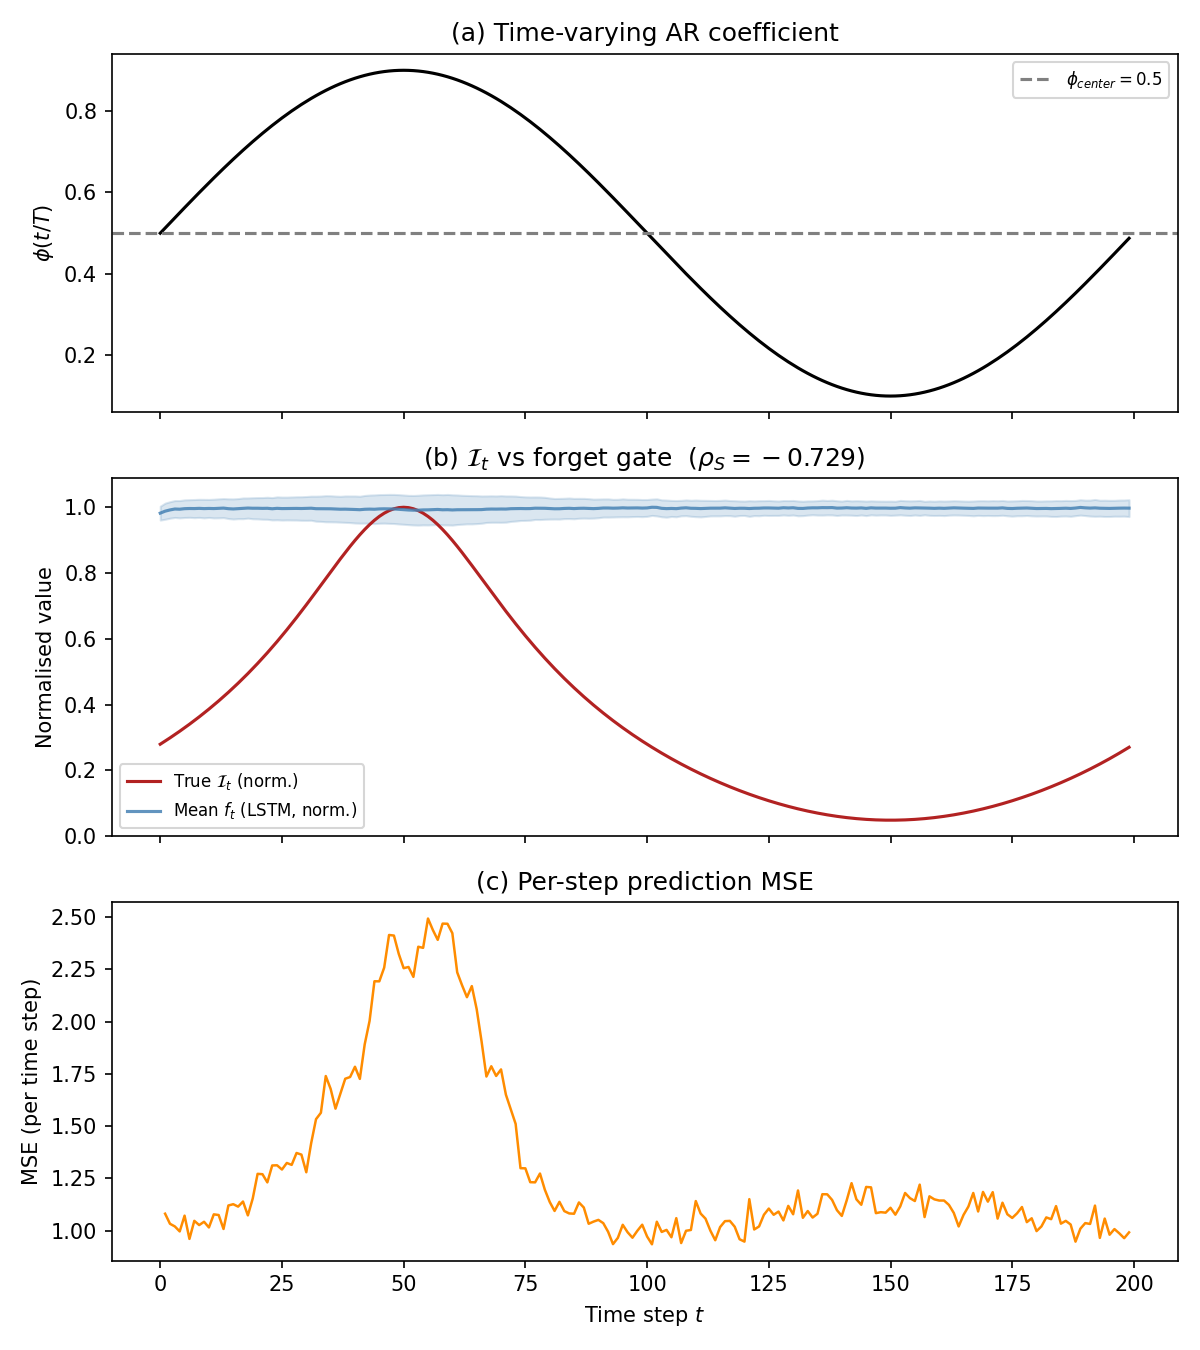
\includegraphics[width=\linewidth]{code/figures/S2A_locally_stationary.png}
\caption{Study S2A: (a) Time-varying $\phi(u)$; (b) normalized true $J(u)$
  (red) vs.\ mean forget gate $\bar f_t$ (blue $\pm$ 1\,s.d.); (c) per-step
  prediction MSE over 1000 locally stationary sequences.
  The forget gate systematically mis-adapts: it moves opposite to $J(u)$,
  yielding the strongly negative Spearman correlation in Table~\ref{tab:supp-S2A}.}
\label{fig:supp-S2A}
\end{figure}

\subsubsection*{Interpretation}

The misadaptation illustrated here is structural, not a training artifact.
Under local stationarity, the optimal forget gate should track the local
persistence $\phi(u)$; a gate trained at a fixed $\phi_{\mathrm{center}}$
has no mechanism to adapt.
This underscores the need for the non-stationarity correction in
\citet{chang2026jrssb}, where KLIEP density-ratio reweighting
\citep{sugiyama2012density} is applied to align the effective training
distribution with the local stationarity regime.

\subsection{Study J-Surr: $J_t$ Surrogate Comparison (Study~S3)}
\label{app:supp-jsurr}

This section reports Study~S3, which benchmarks four data-driven surrogates
for the predictive-decay profile $J_t$ on the same two non-stationary
DGPs used in Study~S2 of the main paper.

\subsubsection*{DGPs and estimators}

Two DGPs are used.
DGP~A is the locally stationary AR(1) of Section~\ref{app:supp-lsdiag} above
($\phi(u) = 0.50 + 0.40\sin(2\pi u)$, smooth variation).
DGP~B is the abrupt change-point AR(1) of Study~S2 in the main paper
($\phi_{\mathrm{before}} = 0.30 \to \phi_{\mathrm{after}} = 0.85$, $\tau^* = 100$).

Four estimators are compared over $N = 500$ independent replications.
The \emph{normalized MSE}
$\mathrm{NMSE} = \mathrm{MSE}(\hat J_t,\,J_t^{\mathrm{true}}) / \mathrm{Var}(J_t^{\mathrm{true}})$
is reported; $\mathrm{NMSE} = 1$ is the trivial baseline.

\subsubsection*{Results}

Table~\ref{tab:supp-S3} and Figure~\ref{fig:supp-S3} summarize the results.
Under smooth non-stationarity (DGP~A), the KLIEP-corrected estimator is the
only method to achieve NMSE $< 1$ (mean 0.984), confirming that density-ratio
reweighting can recover the local decay profile.
Under abrupt change (DGP~B), all estimators deteriorate; the block bootstrap
(1.189) is the only method that meaningfully beats the naive constant (3.000).

\begin{table}[ht]
\centering
\caption{Study S3: Normalized MSE of four $J_t$ estimators.
  Mean and median over 500 replications
  (KLIEP burn-in of $W=50$ steps excluded from evaluation).}
\label{tab:supp-S3}
\begin{tabular}{lcccc}
\toprule
Estimator & \multicolumn{2}{c}{DGP A (LS-AR)} &
            \multicolumn{2}{c}{DGP B (CP-AR)} \\
          & Mean NMSE & Median NMSE & Mean NMSE & Median NMSE \\
\midrule
Naive constant       & 1.004 & 1.004 & 3.000 & 3.000 \\
Forget gate (LSTM)   & 1.017 & 1.016 & 3.011 & 3.010 \\
Block bootstrap      & 1.393 & 1.234 & 1.189 & 1.132 \\
KLIEP-corrected      & \textbf{0.984} & \textbf{0.977} & 2.757 & 2.741 \\
\bottomrule
\end{tabular}
\end{table}

\begin{figure}[H]
\centering
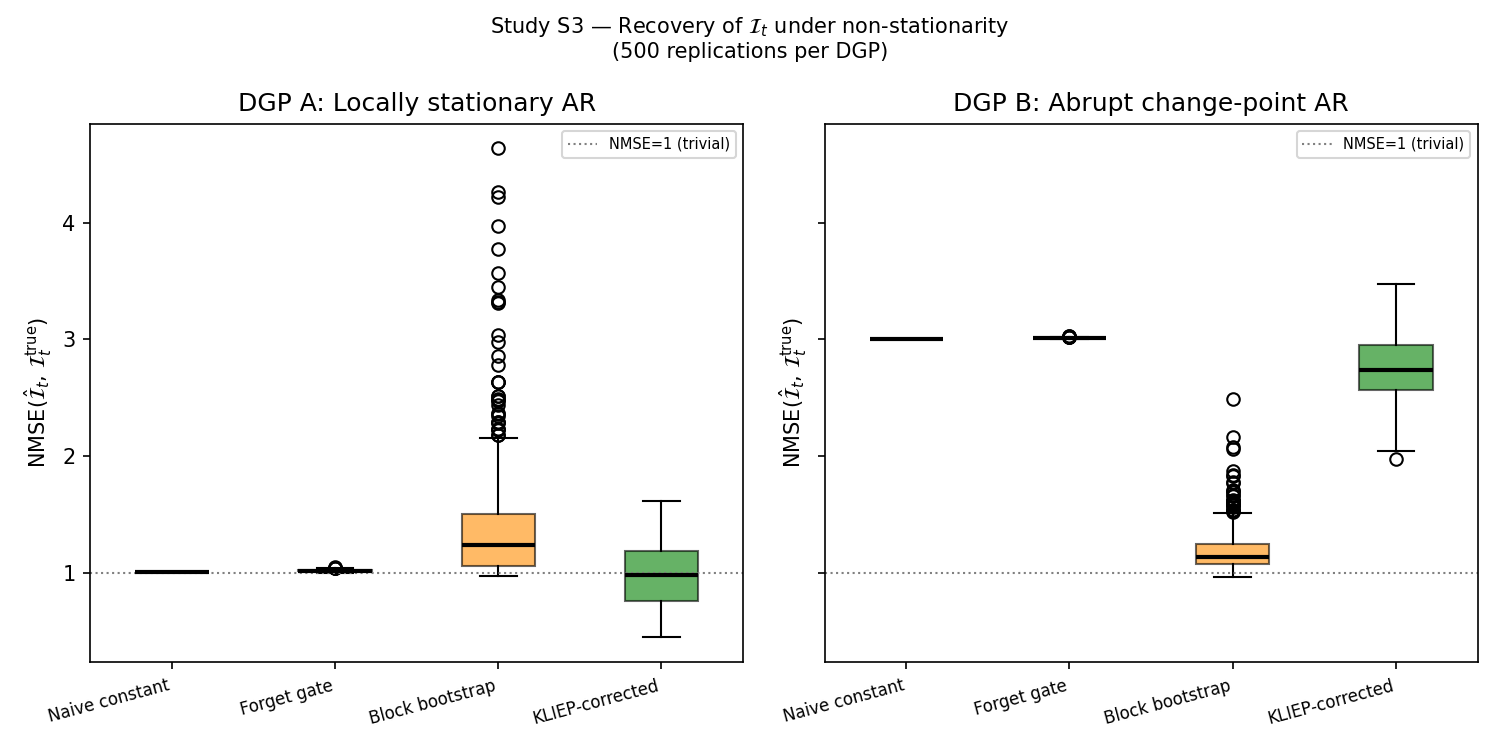
\includegraphics[width=0.95\linewidth]{code/figures/S3_nmse_comparison.png}
\caption{Study S3: NMSE boxplots for four $\hat J_t$ estimators on
  DGP~A (left) and DGP~B (right).
  The dotted line at NMSE$\,=1$ marks the trivial baseline.}
\label{fig:supp-S3}
\end{figure}

\subsubsection*{Interpretation}

Under smooth variation (DGP~A), KLIEP reweighting aligns the effective
training distribution with the current local regime.
Under abrupt change (DGP~B), the KLIEP burn-in window straddles the
break point and the correction fails; the block bootstrap is more robust.
These findings motivate the two-regime strategy in \citet{chang2026jrssb}:
use KLIEP correction in locally stationary windows and switch to block
bootstrap near detected change-points.

% =============================================================================
\bibliographystyle{imsart-nameyear}
\bibliography{P1_references}

\end{document}
